Para a contextualização da ação de controle sobre sistemas não lineares, escolheu-se o sistema de pêndulo invertido por ser análogo ao modelo do \textit{drone}. Esta escolha foi baseada no fato de este sistema ser considerado um problema clássico de sistema não linear instável, sendo retratado repetidamente na literatura, como em \cite[p.~68]{Ogata2010} e em \cite[p.~186]{Dorf2011}, além de ser largamente usado como \textit{benchmark} para comparação de eficiência de variados métodos de controle, sendo alvo de estudo em diversos artigos. O primeiro passo para seu estudo é a sua modelagem matemática.

\subsection{Modelagem Matemática}
\label{subsec:sistemas-pendulum-mathematical-model}

Considerando o diagrama de corpo livre mostrado na \autoref{fig:Ogata2010_inverted_pendulum_diagram_complete}-b e se utilizando de desenvolvimento matemático chegou-se às seguintes equações para descrever o movimento do sistema do pêndulo invertido sobre o carro:
\begin{equation} \label{eq:modeling_pendulum_eq1}
	(M+m)\ddot{x} + ml\ddot{\theta} = u
\end{equation}
\begin{equation} \label{eq:modeling_pendulum_eq2}
	(I+ml^2)\ddot{\theta} + ml\ddot{x} = mlg\theta
\end{equation}
 
Em que $I$ é o momento de inércia da haste.

A partir de manipulação matemática, as equações \ref{eq:modeling_pendulum_eq1} e \ref{eq:modeling_pendulum_eq2} podem ser reescritas como:
\begin{equation} \label{eq:modeling_pendulum_eq1_modified}
	Ml\ddot{\theta} = (M+m)g\theta - u
\end{equation}
\begin{equation} \label{eq:modeling_pendulum_eq2_modified}
	M\ddot{x} = u - mg\theta
\end{equation}

A partir da \autoref{eq:modeling_pendulum_eq2_modified}, \citeonline[p.~71]{Ogata2010} obtém a função de transferência da planta como:
\begin{align} \label{eq:modeling_pendulum_tf}
\frac{\Theta(s)}{-U(s)} &= \frac{1}{Mls^2-(M+m)g} \nonumber \\
						&= \frac{1}{Ml(s+\sqrt{\frac{M+m}{Ml}g})(s-\sqrt{\frac{M+m}{Ml}g})}
\end{align}

Na \autoref{eq:modeling_pendulum_tf}, verifica-se que a planta do pêndulo invertido possui um polo no eixo real negativo e outro no eixo real positivo. Estes polos são: 
\begin{equation} \label{eq:modeling_pendulum_tf_neg_pole}
	s = -\sqrt{\frac{M+m}{Ml}g}
\end{equation}
\begin{equation} \label{eq:modeling_pendulum_tf_pos_pole}
	s = \sqrt{\frac{M+m}{Ml}g}
\end{equation}

Por possuir um polo no eixo real positivo, definido pela \autoref{eq:modeling_pendulum_tf_pos_pole}, a planta é instável em malha aberta.

\subsection{Representação no Espaço de Estados}
\label{subsec:sistemas-inverted-pendulum-state-spaces}
Para a representação do sistema no espaço de estados, em \cite[p.~71]{Ogata2010} as variáveis de estado $x_1$, $x_2$, $x_3$ e $x_4$ foram definidas como:
\begin{align*}
	x_1 &= \theta \\
	x_2 &= \dot{\theta} \\
	x_3 &= x \\
	x_4 &= \dot{x}
\end{align*}

Com isto, se obtém o vetor de estados $X$ definido por:
\begin{equation*}
X=
\left[ \begin{array}{@{}*{4}{c}@{}}
     \theta & \dot{\theta} & x & \dot{x} \\
\end{array} \right]^T
\end{equation*}

Além disto, o vetor $y$ de saída do sistema foi definido como:
\[
	y = 
	\begin{bmatrix}
		y_1 \\
		y_2
	\end{bmatrix} = 
	\begin{bmatrix}
			\theta \\
			x
	\end{bmatrix} =
	\begin{bmatrix}
			x_1\\
			x_3
	\end{bmatrix}
\]

A partir de novas manipulações matemáticas, mostra-se que a representação por espaço de estados deste sistema de pêndulo invertido pode ser definido como:
\begin{align} \label{eq:space_state_equation_pendulum}
	\dot{x} &= Ax + Bu \\
	y		&= Cx + Du
\end{align}

Em que:
\[
	A = 
	\begin{bmatrix}
		0 & 1 & 0 & 0 \\
		\frac{M+m}{Ml}g & 0 & 0 & 0 \\
		0 & 0 & 0 & 1 \\
		-\frac{m}{M}g & 0 & 0 & 0
	\end{bmatrix}\quad
	B = 
	\begin{bmatrix}
		0 \\
		-\frac{1}{Ml} \\
		0 \\
		\frac{1}{Ml}
	\end{bmatrix}
\]

\[
	C = 
		\begin{bmatrix}
			1 & 0 & 0 & 0 \\
			0 & 0 & 1 & 0
		\end{bmatrix}\quad
	D = 
		\begin{bmatrix}
			0 \\
			0
		\end{bmatrix}
\]

Desta forma, se obtém a representação completa do sistema de pêndulo invertido no espaço de estados.

\subsection{Experimentos Realizados}
\label{subsec:metodolgoia-pendulum-experimentos}

Uma variação do algoritmo presente em \cite[p.~750]{Ogata2010} foi usado para simular a resposta do sistema de pêndulo invertido a uma entrada em degrau unitário em duas situações: sem nenhuma ação de controle; e com uma ação de controle tradicional. Neste segundo caso, foi utilizado um servo sistema tipo 1, como mostrado na \autoref{fig:Ogata2010_servo_system_type_1}.

\begin{figure}[!htb]
    \centering
    \caption{Diagrama de blocos representando o sistema de pêndulo invertido controlado por um servo sistema tipo 1}
    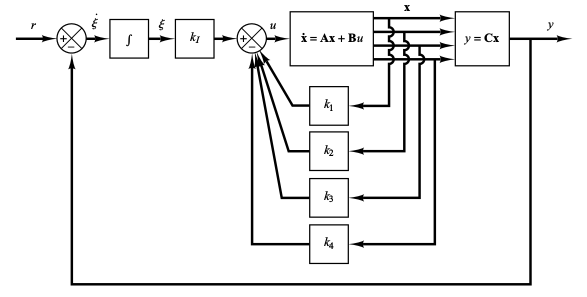
\includegraphics[width=1\textwidth]{./04-figuras/Ogata2010_servo_system_type_1}
    \fonte{\cite[p.~747]{Ogata2010}}
    \label{fig:Ogata2010_servo_system_type_1}
\end{figure}

Os parâmetros do controlador utilizados foram \cite[p.~749]{Ogata2010}:
\[
	k = 
		\begin{bmatrix}
			k_1 &
			k_2 &
			k_3 &
			k_4
		\end{bmatrix} =
		\begin{bmatrix}
			-157,6336 &
			-35,3733 &
			-56,0652 &
			50,9684
		\end{bmatrix}
\]

e
\[
k_I = -50,9684
\]

O algoritmo que implementa o sistema do pêndulo invertido e também o controlador proposto é mostrado no Apêndice \ref{chap:apendicex-pendulum-modelagem-controle}. O intuito desta etapa é mostrar a instabilidade do sistema, que diverge ao sofrer qualquer perturbação, e a ação de controle que estabiliza este sistema, tornando-o estável, fazendo com que ele não mais divirja quando perturbado.

O diagrama de blocos do sistema desenvolvido para representar o pêndulo invertido é mostrado na \autoref{fig:simulink-pendulo-diagrama-geral}. Como se pode ver, este sistema possui uma única entrada, $u$, referente à força aplicada sobre o carro, e quatro saídas: theta ($\theta$) representando o ângulo da haste do pêndulo em relação ao eixo vertical; theta\_dot ($\dot{\theta}$), a taxa de variação deste ângulo; x, a posição do carro sobre o eixo horizontal; e x\_ponto ($\dot{x}$), sua velocidade sobre este mesmo eixo.

\begin{figure}[!htb]
    \centering
    \caption{Diagrama de blocos representando o sistema de pêndulo invertido}
    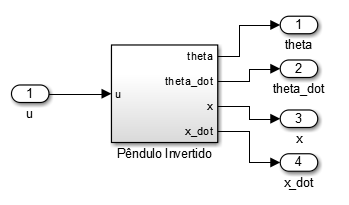
\includegraphics[width=.6\textwidth]{./04-figuras/simulink_pendulo/diagrama_geral}
    \label{fig:simulink-pendulo-diagrama-geral}
\end{figure}

A estrutura do primeiro experimento realizado é mostrado na \autoref{fig:simulink-pendulo-diagrama-geral-step}. Como se pode ver, foi aplicada à entrada $u$ do sistema, uma entrada em degrau unitário. Neste experimento, são verificadas as resposta de todas as saídas a esta excitação na entrada. Para permitir uma clara distinção da resposta do sistema sem a excitação e com ela, foi definido que ela ocorresse no tempo $t=10\ s$.

\begin{figure}[!htb]
    \centering
    \caption{Diagrama de blocos representando experimento realizado com o sistema de pêndulo invertido}
    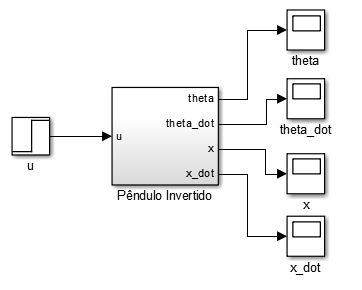
\includegraphics[width=.6\textwidth]{./04-figuras/simulink_pendulo/diagrama_step_u}
    \label{fig:simulink-pendulo-diagrama-geral-step}
\end{figure}

A estrutura do segundo experimento é análoga à do primeiro. Uma excitação em degrau é aplicada na entrada e todos os estados são verificados. Para este experimento, entretanto, a estrutura inclui um servo sistema tipo um, como mostrado na \autoref{fig:Ogata2010_servo_system_type_1},  para estabilizar o pêndulo.
